\documentclass{article}\usepackage[]{graphicx}\usepackage[]{color}
% maxwidth is the original width if it is less than linewidth
% otherwise use linewidth (to make sure the graphics do not exceed the margin)
\makeatletter
\def\maxwidth{ %
  \ifdim\Gin@nat@width>\linewidth
    \linewidth
  \else
    \Gin@nat@width
  \fi
}
\makeatother

\definecolor{fgcolor}{rgb}{0.345, 0.345, 0.345}
\newcommand{\hlnum}[1]{\textcolor[rgb]{0.686,0.059,0.569}{#1}}%
\newcommand{\hlstr}[1]{\textcolor[rgb]{0.192,0.494,0.8}{#1}}%
\newcommand{\hlcom}[1]{\textcolor[rgb]{0.678,0.584,0.686}{\textit{#1}}}%
\newcommand{\hlopt}[1]{\textcolor[rgb]{0,0,0}{#1}}%
\newcommand{\hlstd}[1]{\textcolor[rgb]{0.345,0.345,0.345}{#1}}%
\newcommand{\hlkwa}[1]{\textcolor[rgb]{0.161,0.373,0.58}{\textbf{#1}}}%
\newcommand{\hlkwb}[1]{\textcolor[rgb]{0.69,0.353,0.396}{#1}}%
\newcommand{\hlkwc}[1]{\textcolor[rgb]{0.333,0.667,0.333}{#1}}%
\newcommand{\hlkwd}[1]{\textcolor[rgb]{0.737,0.353,0.396}{\textbf{#1}}}%
\let\hlipl\hlkwb

\usepackage{framed}
\makeatletter
\newenvironment{kframe}{%
 \def\at@end@of@kframe{}%
 \ifinner\ifhmode%
  \def\at@end@of@kframe{\end{minipage}}%
  \begin{minipage}{\columnwidth}%
 \fi\fi%
 \def\FrameCommand##1{\hskip\@totalleftmargin \hskip-\fboxsep
 \colorbox{shadecolor}{##1}\hskip-\fboxsep
     % There is no \\@totalrightmargin, so:
     \hskip-\linewidth \hskip-\@totalleftmargin \hskip\columnwidth}%
 \MakeFramed {\advance\hsize-\width
   \@totalleftmargin\z@ \linewidth\hsize
   \@setminipage}}%
 {\par\unskip\endMakeFramed%
 \at@end@of@kframe}
\makeatother

\definecolor{shadecolor}{rgb}{.97, .97, .97}
\definecolor{messagecolor}{rgb}{0, 0, 0}
\definecolor{warningcolor}{rgb}{1, 0, 1}
\definecolor{errorcolor}{rgb}{1, 0, 0}
\newenvironment{knitrout}{}{} % an empty environment to be redefined in TeX

\usepackage{alltt}

\usepackage{amsmath}
\usepackage{hyperref}
\usepackage[round]{natbib}
\bibliographystyle{unsrtnat}

% \usepackage[backend=bibtex, style=authoryear-icompm, natbib=true]{biblatex}
% \addbibresource{bib-packages.bib}

% \bibliographystyle{plainnat}
% \usepackage{natbib}
% \addbibresource{bib_packages.bib}
% \addbibresource{bib-packages.bib}
\DeclareMathOperator*{\argmin}{argmin}
\IfFileExists{upquote.sty}{\usepackage{upquote}}{}
\begin{document}









\section{Introduction}

In this project the \href{https://github.com/karlrupp/microprocessor-trend-data/tree/master/42yrs}{frequency dataset} is analysed. The frequency dataset consists of 90 observations of microprocessor frequencies between 1971 and 2018 (Figure \ref{fig:plot1}).

\begin{figure}
\begin{knitrout}
\definecolor{shadecolor}{rgb}{0.969, 0.969, 0.969}\color{fgcolor}\begin{kframe}
\begin{alltt}
\hlstd{data} \hlkwb{<-} \hlkwd{read.table}\hlstd{(}\hlstr{"../../frequency.dat"}\hlstd{)}
\hlkwd{names}\hlstd{(data)} \hlkwb{<-} \hlkwd{c}\hlstd{(}\hlstr{"year"}\hlstd{,} \hlstr{"freq"}\hlstd{)}
\hlkwd{plot}\hlstd{(freq} \hlopt{~} \hlstd{year,} \hlkwc{data} \hlstd{= data,} \hlkwc{ylab} \hlstd{=} \hlstr{"Freqency [MHz]"}\hlstd{,}
    \hlkwc{ylim} \hlstd{=} \hlkwd{c}\hlstd{(}\hlopt{-}\hlnum{1000}\hlstd{,} \hlnum{6000}\hlstd{))}
\end{alltt}
\end{kframe}

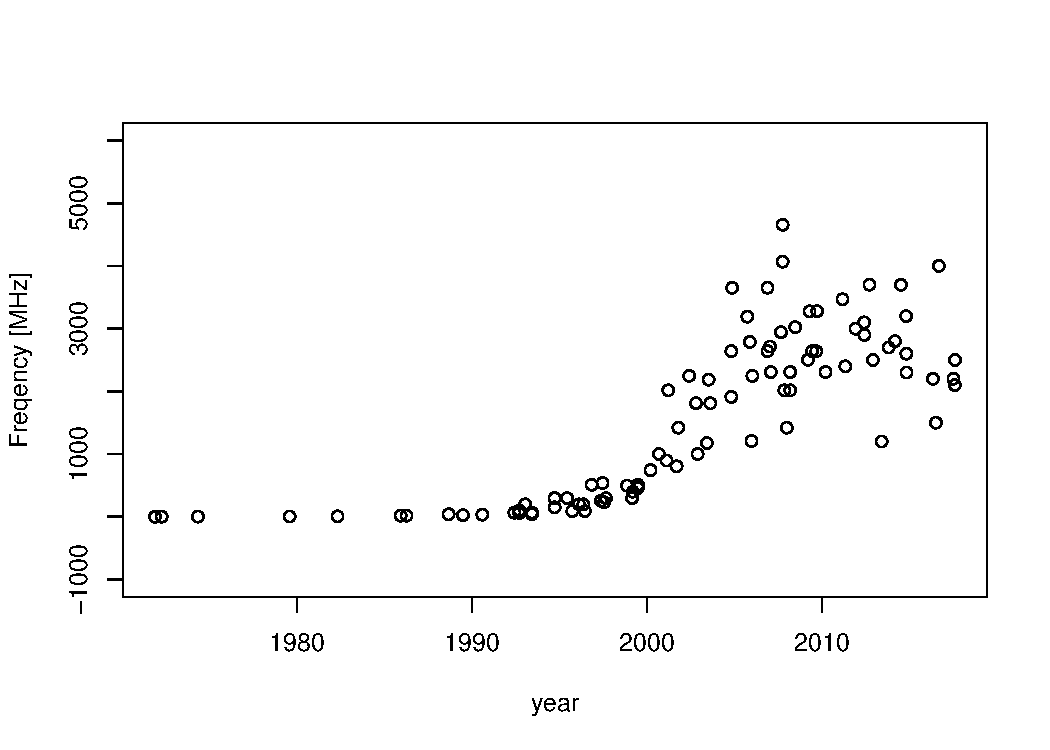
\includegraphics[width=1\linewidth]{figure/plot1-1} \hfill{}



\end{knitrout}
\caption{Microprocessor frequencies between 1971 and 2018.}
\label{fig:plot1}
\end{figure}


A first inspection of the data shows relatively low frequencies in the beginning with a sudden increase arround the year 1995. The fastest increase we see arround the year 2002, afterwards the frequency starts leveling off. This pattern is characteristic for logistic functions, which might be useful to model the data.

The variability increases with the level of frequency (heteroscedasticity) and all frequencies are naturally positive. Therefore, a log transformation might be useful to stabilize the variance.


\begin{figure}
\begin{knitrout}
\definecolor{shadecolor}{rgb}{0.969, 0.969, 0.969}\color{fgcolor}\begin{kframe}
\begin{alltt}
\hlkwd{plot}\hlstd{(}\hlkwd{log}\hlstd{(freq)} \hlopt{~} \hlstd{year,} \hlkwc{data} \hlstd{= data,} \hlkwc{ylab} \hlstd{=} \hlstr{"log(Freqency)"}\hlstd{)}
\end{alltt}
\end{kframe}

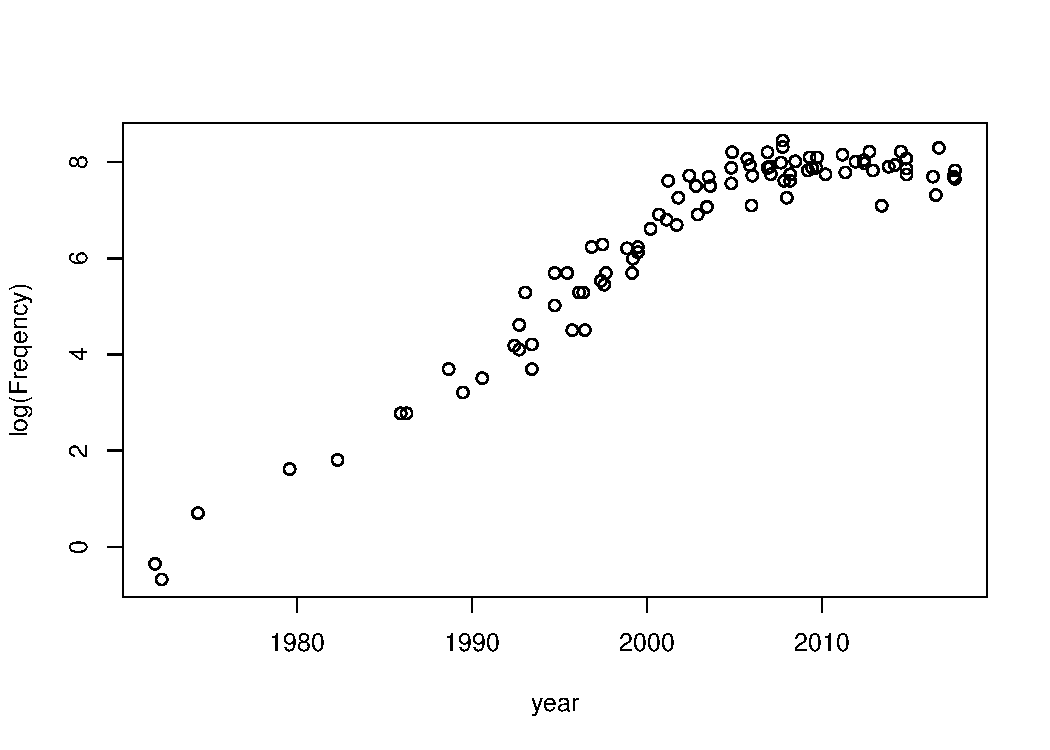
\includegraphics[width=1\linewidth]{figure/plot2-1} \hfill{}



\end{knitrout}
\caption{Microprocessor frequencies between 1971 and 2018 on log scale.}
\label{fig:plot2}
\end{figure}


The log transformed frequencies have a relatively stable variance over all years (Figure \ref{fig:plot2}). There is a clear increase in log frequency until the year 2005. Afterwards the log frequency seems to be relatively stable. A piecewise linear function might be a good choice to model these data.


\section{Model fitting and prediction}

\subsection{Model}

Closesly related to piecewise linear functions are regression splines. Splines are picewise polynomials which are continuously differentiable up to a certain degree at the nodes. Splines can easliy be fitted with a generalized additive model (GAM). The model can be written as

\begin{equation}
g(E(Y)) = \beta_0 + f_1(x_1) + f_2(x_2) + \dots + f_m(x_m)
\end{equation}

where $g(\cdot)$ is a link function, linking the expected value of $Y$ to the linear predictor and $f_i(\cdot)$ are smooth functions of the predictor $x_i$. The predictor is a linear combination of smooth functions $f_i(\cdot)$. The smooth function makes GAM more general than generalized linear models but they do not allow automatically for interactions (no curse of dimensionality). In our case we use splines as smooth functions.

The degrees of freedom of the spline have to be limited to avoid overfitting. This is done by penalizing the wiggliness of the spline in the loss function

\begin{equation}
\hat{f} = \argmin_{f \in F} \sum_{i=1}^n(y_i - f(x_i))^2 + \lambda \int_{a}^bg''(x)^2 dx
\end{equation}

where $F$ is the class of possible spline functions, $\lambda$ is the penalty parameter, $a$ and $b$ are the lower and upper boundary of the range of $x$, respectively. The implementation of GAM in R with the function `gam()`, automatically chooses the penalty parameter with cross validation.

Applying the model to the frequency data leads to

\begin{equation}
E(\log(Frequency)) = \beta_0 + f_{t}(t)
\end{equation}

which means our $g(\cdot)$ is the identity function and we have only one smooth spline function for our predictor time $t$.


\subsection{Fitting}

We fit a GAM to the data using the function \texttt{gam()} of the package \texttt{mgcv} \citep{R-mgcv}.

\begin{knitrout}
\definecolor{shadecolor}{rgb}{0.969, 0.969, 0.969}\color{fgcolor}\begin{kframe}
\begin{alltt}
\hlcom{# packages}
\hlcom{# ----------------------------------------------------------------}
\hlkwd{library}\hlstd{(mgcv)}
\end{alltt}
\end{kframe}
\end{knitrout}

\begin{figure}
\begin{knitrout}
\definecolor{shadecolor}{rgb}{0.969, 0.969, 0.969}\color{fgcolor}\begin{kframe}
\begin{alltt}
\hlstd{fit} \hlkwb{<-} \hlkwd{gam}\hlstd{(}\hlkwd{log}\hlstd{(freq)} \hlopt{~} \hlkwd{s}\hlstd{(year),} \hlkwc{data} \hlstd{= data)}
\hlkwd{plot}\hlstd{(}\hlkwd{log}\hlstd{(freq)} \hlopt{~} \hlstd{year,} \hlkwc{data} \hlstd{= data,} \hlkwc{ylab} \hlstd{=} \hlstr{"log(freqency)"}\hlstd{)}
\hlkwd{lines}\hlstd{(data}\hlopt{$}\hlstd{year,} \hlkwd{predict}\hlstd{(fit),} \hlkwc{col} \hlstd{=} \hlstr{"red"}\hlstd{,} \hlkwc{lwd} \hlstd{=} \hlnum{2}\hlstd{)}
\end{alltt}
\end{kframe}

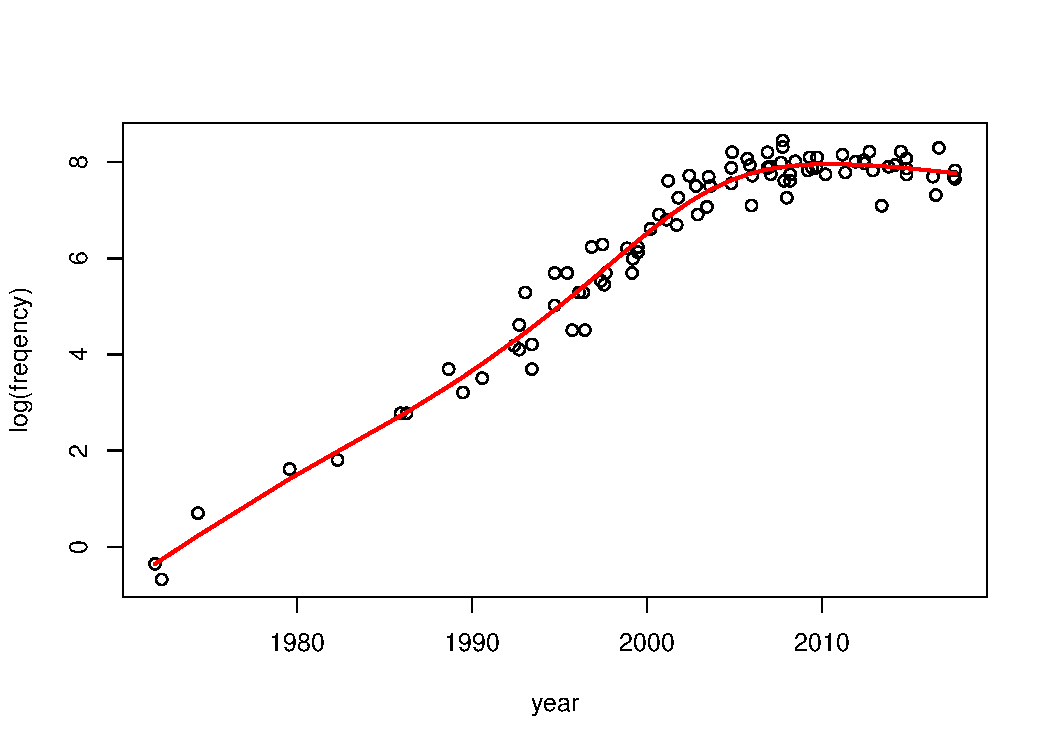
\includegraphics[width=1\linewidth]{figure/plot3-1} \hfill{}



\end{knitrout}
\caption{Fitted GAM model.}
\label{fig:plot3}
\end{figure}


GAM is able to follow the trend without overfitting to the single observations (Figure \ref{fig:plot3}).



\begin{knitrout}
\definecolor{shadecolor}{rgb}{0.969, 0.969, 0.969}\color{fgcolor}\begin{kframe}
\begin{alltt}
\hlkwd{summary}\hlstd{(fit)}
\end{alltt}
\begin{verbatim}

Family: gaussian 
Link function: identity 

Formula:
log(freq) ~ s(year)

Parametric coefficients:
            Estimate Std. Error t value Pr(>|t|)    
(Intercept)  6.45383    0.03913     165   <2e-16 ***
---
Signif. codes:  0 '***' 0.001 '**' 0.01 '*' 0.05 '.' 0.1 ' ' 1

Approximate significance of smooth terms:
          edf Ref.df     F p-value    
s(year) 5.266  6.378 413.3  <2e-16 ***
---
Signif. codes:  0 '***' 0.001 '**' 0.01 '*' 0.05 '.' 0.1 ' ' 1

R-sq.(adj) =  0.967   Deviance explained = 96.9%
GCV = 0.14808  Scale est. = 0.13777   n = 90
\end{verbatim}
\end{kframe}
\end{knitrout}


The predictor year is highly significant with 5.266 estimated degrees of freedom.


\subsection{Validation}

The Tukey-Anscombe plot and the QQ plot of the model fit shows that the model assumptions are largely fulfilled (Figure \ref{fig:plot4}). The variance stays constant over the entire range of fitted value and the residuals follow a normal distribution.

\begin{figure}
\begin{knitrout}
\definecolor{shadecolor}{rgb}{0.969, 0.969, 0.969}\color{fgcolor}\begin{kframe}
\begin{alltt}
\hlkwd{par}\hlstd{(}\hlkwc{mfrow} \hlstd{=} \hlkwd{c}\hlstd{(}\hlnum{1}\hlstd{,} \hlnum{2}\hlstd{))}
\hlkwd{with}\hlstd{(fit,} \hlkwd{plot}\hlstd{(fitted.values, residuals))}
\hlkwd{qq.gam}\hlstd{(fit)}
\end{alltt}
\end{kframe}

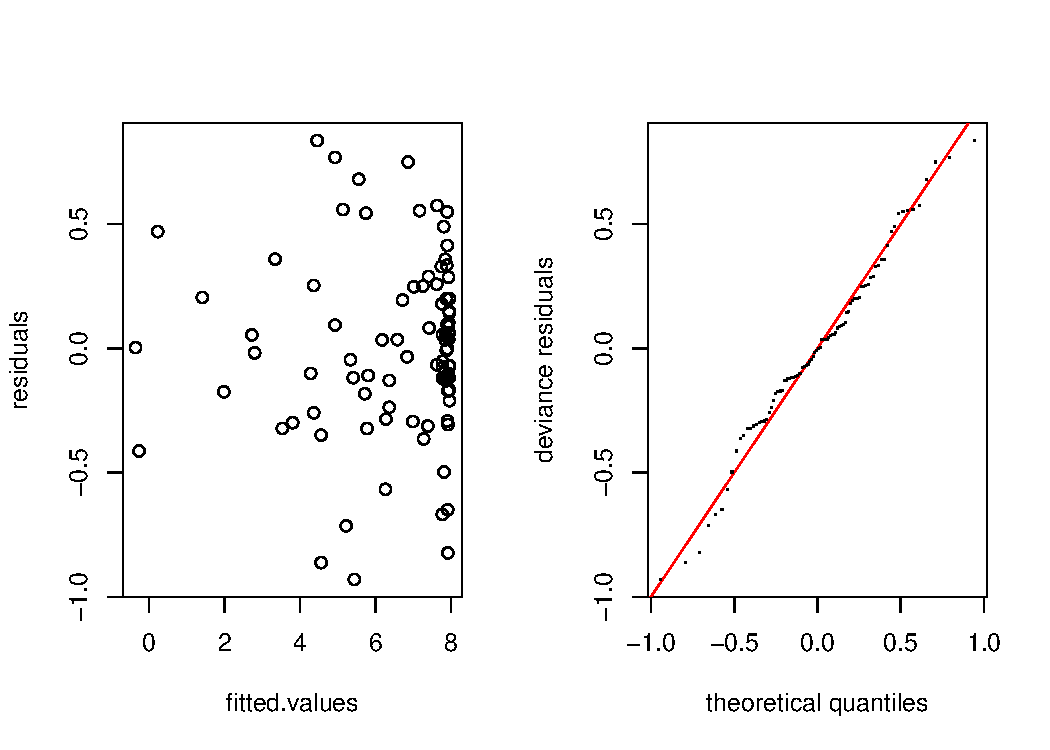
\includegraphics[width=1\linewidth]{figure/plot4-1} \hfill{}



\end{knitrout}
\caption{Residual analysis of the fitted GAM model with Tukey-anscombe plot (left) and QQ plot (right).}
\label{fig:plot4}
\end{figure}



\subsection{Extrapolation}

GAM can also be used to predict future frequencies (Figure \ref{fig:plot5}).


\begin{figure}
\begin{knitrout}
\definecolor{shadecolor}{rgb}{0.969, 0.969, 0.969}\color{fgcolor}\begin{kframe}
\begin{alltt}
\hlkwd{plot}\hlstd{(}\hlkwd{log}\hlstd{(freq)} \hlopt{~} \hlstd{year,} \hlkwc{data} \hlstd{= data,} \hlkwc{ylab} \hlstd{=} \hlstr{"Freqency [MHz]"}\hlstd{,}
    \hlkwc{xlim} \hlstd{=} \hlkwd{c}\hlstd{(}\hlnum{1970}\hlstd{,} \hlnum{2050}\hlstd{),} \hlkwc{ylim} \hlstd{=} \hlkwd{c}\hlstd{(}\hlnum{0}\hlstd{,} \hlnum{10}\hlstd{))}
\hlkwd{lines}\hlstd{(data}\hlopt{$}\hlstd{year,} \hlkwd{predict}\hlstd{(fit),} \hlkwc{col} \hlstd{=} \hlstr{"red"}\hlstd{,} \hlkwc{lwd} \hlstd{=} \hlnum{2}\hlstd{)}
\hlstd{pred_period} \hlkwb{<-} \hlnum{2018}\hlopt{:}\hlnum{2050}
\hlstd{mypred} \hlkwb{<-} \hlkwd{predict.gam}\hlstd{(fit,} \hlkwc{newdata} \hlstd{=} \hlkwd{list}\hlstd{(}\hlkwc{year} \hlstd{= pred_period),}
    \hlkwc{se.fit} \hlstd{= T)}
\hlkwd{polygon}\hlstd{(}\hlkwc{x} \hlstd{=} \hlkwd{c}\hlstd{(pred_period,} \hlkwd{rev}\hlstd{(pred_period)),}
    \hlkwc{y} \hlstd{=} \hlkwd{c}\hlstd{(mypred}\hlopt{$}\hlstd{fit} \hlopt{-} \hlnum{1.96} \hlopt{*} \hlstd{mypred}\hlopt{$}\hlstd{se.fit,} \hlkwd{rev}\hlstd{(mypred}\hlopt{$}\hlstd{fit} \hlopt{+}
        \hlnum{1.96} \hlopt{*} \hlstd{mypred}\hlopt{$}\hlstd{se.fit)),} \hlkwc{border} \hlstd{=} \hlnum{NA}\hlstd{,} \hlkwc{col} \hlstd{=} \hlstr{"lightgray"}\hlstd{)}
\hlkwd{lines}\hlstd{(pred_period, mypred}\hlopt{$}\hlstd{fit,} \hlkwc{col} \hlstd{=} \hlstr{"gray"}\hlstd{,} \hlkwc{lwd} \hlstd{=} \hlnum{2}\hlstd{)}
\end{alltt}
\end{kframe}

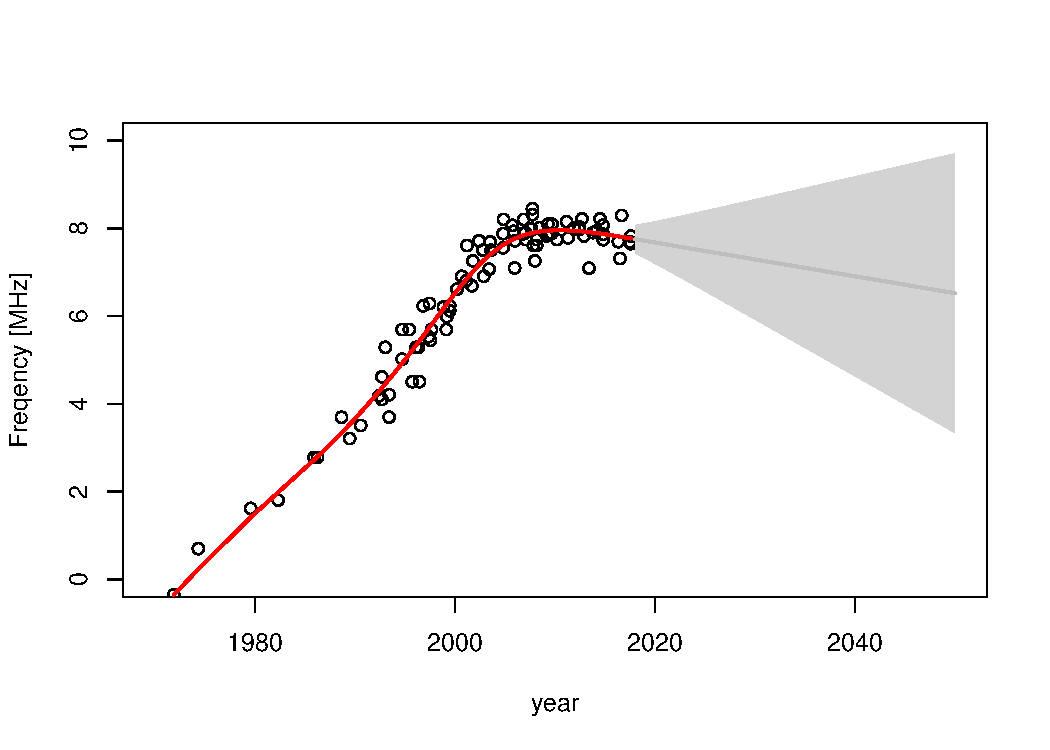
\includegraphics[width=1\linewidth]{figure/plot5-1} \hfill{}



\end{knitrout}
\caption{Linear extrapolation of the trend fitted by the GAM model. The gray area indicate the 95\% CI for the trend prediction.}
\label{fig:plot5}
\end{figure}





\section{Simulation study}

First, I created a true model which can lead to similar data as we observed. I used a logistic model with normally distributed heteroscadistic errors.

\begin{figure}
\begin{knitrout}
\definecolor{shadecolor}{rgb}{0.969, 0.969, 0.969}\color{fgcolor}\begin{kframe}
\begin{alltt}
\hlcom{# Single example}
\hlcom{# ----------------------------------------------------------}
\hlkwd{plot}\hlstd{(freq} \hlopt{~} \hlstd{year,} \hlkwc{data} \hlstd{= data,} \hlkwc{ylab} \hlstd{=} \hlstr{"Freqency [MHz]"}\hlstd{,}
    \hlkwc{ylim} \hlstd{=} \hlkwd{c}\hlstd{(}\hlopt{-}\hlnum{1000}\hlstd{,} \hlnum{6000}\hlstd{))}
\hlcom{# Assume a true function}
\hlstd{fpl} \hlkwb{<-} \hlkwa{function}\hlstd{(}\hlkwc{x}\hlstd{,} \hlkwc{A} \hlstd{=} \hlnum{0}\hlstd{,} \hlkwc{B} \hlstd{=} \hlnum{3000}\hlstd{,} \hlkwc{xmid} \hlstd{=} \hlnum{2003}\hlstd{,}
    \hlkwc{scal} \hlstd{=} \hlnum{3}\hlstd{) \{}
    \hlstd{A} \hlopt{+} \hlstd{(B} \hlopt{-} \hlstd{A)}\hlopt{/}\hlstd{(}\hlnum{1} \hlopt{+} \hlkwd{exp}\hlstd{((xmid} \hlopt{-} \hlstd{x)}\hlopt{/}\hlstd{scal))}
\hlstd{\}}
\hlkwd{curve}\hlstd{(fpl,} \hlkwc{from} \hlstd{=} \hlnum{1970}\hlstd{,} \hlkwc{to} \hlstd{=} \hlnum{2020}\hlstd{,} \hlkwc{add} \hlstd{= T)}
\hlcom{# sample new points}
\hlkwd{set.seed}\hlstd{(}\hlnum{1}\hlstd{)}
\hlstd{true_value} \hlkwb{<-} \hlkwd{fpl}\hlstd{(data}\hlopt{$}\hlstd{year)}
\hlstd{value} \hlkwb{<-} \hlkwd{abs}\hlstd{(true_value} \hlopt{+} \hlkwd{rnorm}\hlstd{(}\hlkwd{length}\hlstd{(true_value),}
    \hlkwc{mean} \hlstd{=} \hlnum{0}\hlstd{,} \hlkwc{sd} \hlstd{= true_value}\hlopt{/}\hlnum{3}\hlstd{))}
\hlstd{sim_data} \hlkwb{<-} \hlkwd{data.frame}\hlstd{(}\hlkwc{year} \hlstd{= data}\hlopt{$}\hlstd{year,} \hlkwc{freq} \hlstd{= value)}
\hlkwd{points}\hlstd{(sim_data}\hlopt{$}\hlstd{year, sim_data}\hlopt{$}\hlstd{freq,} \hlkwc{col} \hlstd{=} \hlstr{"green"}\hlstd{)}
\hlkwd{legend}\hlstd{(}\hlstr{"topleft"}\hlstd{,} \hlkwc{legend} \hlstd{=} \hlkwd{c}\hlstd{(}\hlstr{"Original observations"}\hlstd{,}
    \hlstr{"Observations with new model"}\hlstd{),} \hlkwc{pch} \hlstd{=} \hlnum{1}\hlstd{,} \hlkwc{col} \hlstd{=} \hlkwd{c}\hlstd{(}\hlstr{"black"}\hlstd{,}
    \hlstr{"green"}\hlstd{))}
\end{alltt}
\end{kframe}

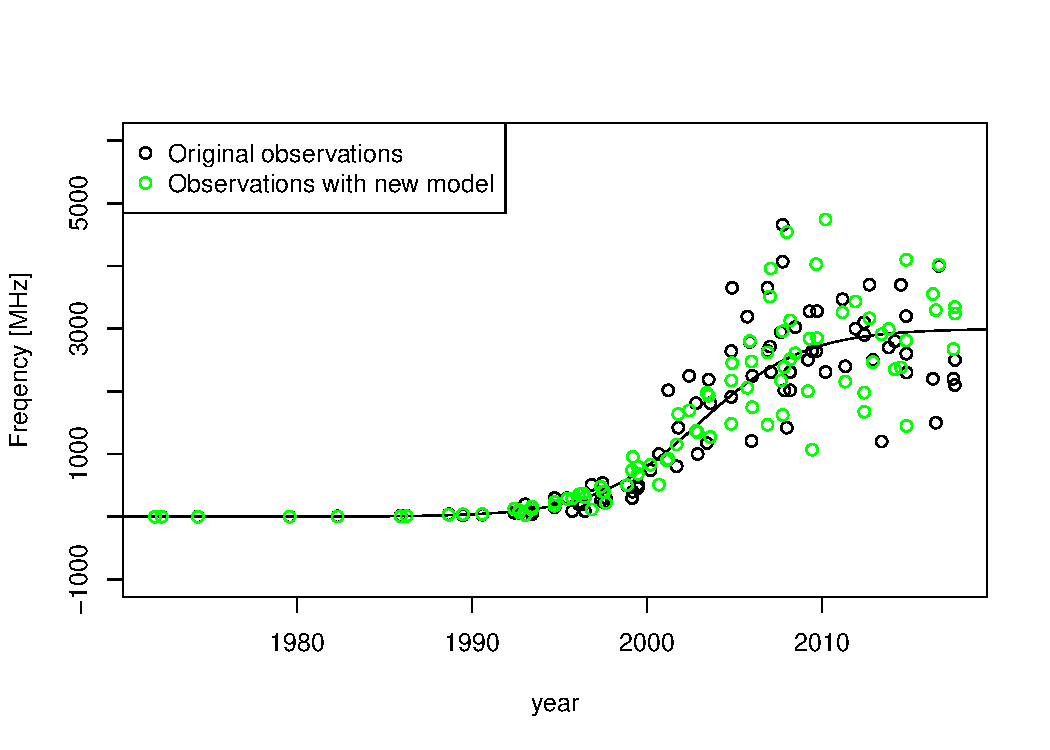
\includegraphics[width=1\linewidth]{figure/plot6-1} \hfill{}



\end{knitrout}
\caption{Random observations using the new model. The black line shows the true mean of the new model.}
\label{fig:plot6}
\end{figure}



Next we fit two models to the new data. One model is a GAM which I already used before, the other is a logistic model fitted with nonlinear least squares.


\begin{figure}
\begin{knitrout}
\definecolor{shadecolor}{rgb}{0.969, 0.969, 0.969}\color{fgcolor}\begin{kframe}
\begin{alltt}
\hlcom{# fit with GAM}
\hlstd{fit} \hlkwb{<-} \hlkwd{gam}\hlstd{(}\hlkwd{log}\hlstd{(freq)} \hlopt{~} \hlkwd{s}\hlstd{(year),} \hlkwc{data} \hlstd{= sim_data)}
\hlcom{# fit with SSfpl()}
\hlstd{fit_ssfpl} \hlkwb{<-} \hlkwd{nls}\hlstd{(freq} \hlopt{~} \hlkwd{SSfpl}\hlstd{(year, A, B, xmid,}
    \hlstd{scal),} \hlkwc{data} \hlstd{= sim_data)}
\hlcom{# plot all}
\hlkwd{plot}\hlstd{(freq} \hlopt{~} \hlstd{year,} \hlkwc{data} \hlstd{= sim_data,} \hlkwc{ylab} \hlstd{=} \hlstr{"Freqency [MHz]"}\hlstd{,}
    \hlkwc{ylim} \hlstd{=} \hlkwd{c}\hlstd{(}\hlopt{-}\hlnum{1000}\hlstd{,} \hlnum{6000}\hlstd{))}
\hlkwd{lines}\hlstd{(sim_data}\hlopt{$}\hlstd{year,} \hlkwd{exp}\hlstd{(}\hlkwd{predict}\hlstd{(fit)),} \hlkwc{col} \hlstd{=} \hlstr{"red"}\hlstd{,}
    \hlkwc{lwd} \hlstd{=} \hlnum{2}\hlstd{)}
\hlkwd{lines}\hlstd{(sim_data}\hlopt{$}\hlstd{year,} \hlkwd{predict}\hlstd{(fit_ssfpl),} \hlkwc{col} \hlstd{=} \hlstr{"green"}\hlstd{,}
    \hlkwc{lwd} \hlstd{=} \hlnum{2}\hlstd{)}
\hlkwd{curve}\hlstd{(fpl,} \hlkwc{lwd} \hlstd{=} \hlnum{2}\hlstd{,} \hlkwc{add} \hlstd{= T)}
\hlkwd{legend}\hlstd{(}\hlstr{"topleft"}\hlstd{,} \hlkwc{legend} \hlstd{=} \hlkwd{c}\hlstd{(}\hlstr{"True model"}\hlstd{,} \hlstr{"GAM fit"}\hlstd{,}
    \hlstr{"FPL fit"}\hlstd{),} \hlkwc{lwd} \hlstd{=} \hlnum{2}\hlstd{,} \hlkwc{col} \hlstd{=} \hlkwd{c}\hlstd{(}\hlstr{"black"}\hlstd{,} \hlstr{"red"}\hlstd{,}
    \hlstr{"green"}\hlstd{))}
\hlkwd{abline}\hlstd{(}\hlkwc{v} \hlstd{=} \hlnum{2008}\hlstd{,} \hlkwc{lty} \hlstd{=} \hlnum{2}\hlstd{)}
\hlkwd{abline}\hlstd{(}\hlkwc{v} \hlstd{=} \hlnum{2017}\hlstd{,} \hlkwc{lty} \hlstd{=} \hlnum{2}\hlstd{)}
\end{alltt}
\end{kframe}

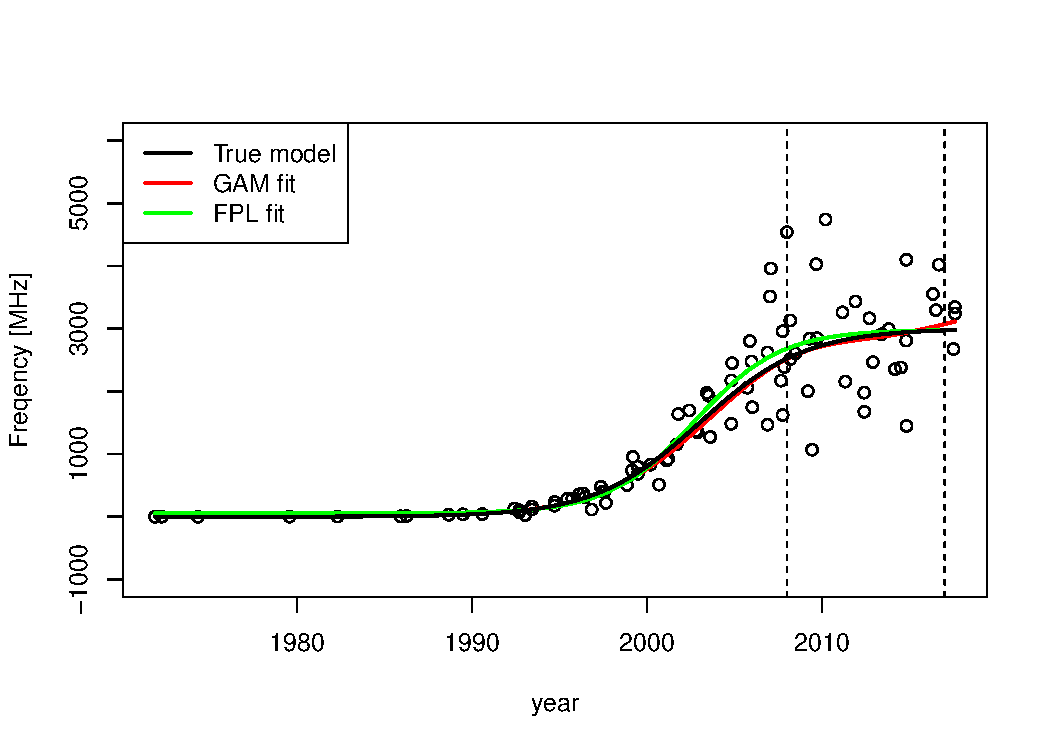
\includegraphics[width=1\linewidth]{figure/plot7-1} \hfill{}



\end{knitrout}
\caption{GAM and four paramteric logistic model (FPL model) fitted to a random sample of the new model.}
\label{fig:plot7}
\end{figure}


To compare how well the two models fit at year 2008 and 2017, we repeat the simulation 1000 times and plot the density of the difference to the true model.

\begin{figure}
\begin{knitrout}
\definecolor{shadecolor}{rgb}{0.969, 0.969, 0.969}\color{fgcolor}\begin{kframe}
\begin{alltt}
\hlcom{# simulation}
\hlcom{# --------------------------------------------------------------}
\hlstd{sim_diff} \hlkwb{<-} \hlkwa{function}\hlstd{() \{}
    \hlstd{true_value} \hlkwb{<-} \hlkwd{fpl}\hlstd{(data}\hlopt{$}\hlstd{year)}
    \hlstd{value} \hlkwb{<-} \hlkwd{abs}\hlstd{(true_value} \hlopt{+} \hlkwd{rnorm}\hlstd{(}\hlkwd{length}\hlstd{(true_value),}
        \hlkwc{mean} \hlstd{=} \hlnum{0}\hlstd{,} \hlkwc{sd} \hlstd{= true_value}\hlopt{/}\hlnum{3}\hlstd{))}
    \hlstd{sim_data} \hlkwb{<-} \hlkwd{data.frame}\hlstd{(}\hlkwc{year} \hlstd{= data}\hlopt{$}\hlstd{year,} \hlkwc{freq} \hlstd{= value)}
    \hlstd{fit} \hlkwb{<-} \hlkwd{gam}\hlstd{(}\hlkwd{log}\hlstd{(freq)} \hlopt{~} \hlkwd{s}\hlstd{(year),} \hlkwc{data} \hlstd{= sim_data)}
    \hlstd{fit_ssfpl} \hlkwb{<-} \hlkwd{nls}\hlstd{(freq} \hlopt{~} \hlkwd{SSfpl}\hlstd{(year, A, B,}
        \hlstd{xmid, scal),} \hlkwc{data} \hlstd{= sim_data)}
    \hlstd{gam_pred} \hlkwb{<-} \hlkwd{unname}\hlstd{(}\hlkwd{exp}\hlstd{(}\hlkwd{predict}\hlstd{(fit,} \hlkwc{newdata} \hlstd{=} \hlkwd{list}\hlstd{(}\hlkwc{year} \hlstd{=} \hlkwd{c}\hlstd{(}\hlnum{2008}\hlstd{,}
        \hlnum{2017}\hlstd{)))))}
    \hlstd{ssfpl_pred} \hlkwb{<-} \hlkwd{predict}\hlstd{(fit_ssfpl,} \hlkwc{newdata} \hlstd{=} \hlkwd{list}\hlstd{(}\hlkwc{year} \hlstd{=} \hlkwd{c}\hlstd{(}\hlnum{2008}\hlstd{,}
        \hlnum{2017}\hlstd{)))}
    \hlstd{true_values} \hlkwb{<-} \hlkwd{fpl}\hlstd{(}\hlkwd{c}\hlstd{(}\hlnum{2008}\hlstd{,} \hlnum{2017}\hlstd{))}
    \hlkwd{c}\hlstd{(gam_pred} \hlopt{-} \hlstd{true_values, ssfpl_pred} \hlopt{-} \hlstd{true_values)}
\hlstd{\}}
\hlstd{out} \hlkwb{<-} \hlkwd{replicate}\hlstd{(}\hlnum{1000}\hlstd{,} \hlkwd{sim_diff}\hlstd{())}
\hlstd{out} \hlkwb{<-} \hlkwd{t}\hlstd{(out)}
\hlcom{# plot simulation results}
\hlcom{# -------------------------------------------------}
\hlkwd{plot}\hlstd{(}\hlkwd{density}\hlstd{(out[,} \hlnum{1}\hlstd{]),} \hlkwc{main} \hlstd{=} \hlstr{"Difference to true function at 2008"}\hlstd{,}
    \hlkwc{xlim} \hlstd{=} \hlkwd{c}\hlstd{(}\hlopt{-}\hlnum{1000}\hlstd{,} \hlnum{1000}\hlstd{),} \hlkwc{ylim} \hlstd{=} \hlkwd{c}\hlstd{(}\hlnum{0}\hlstd{,} \hlnum{0.005}\hlstd{),}
    \hlkwc{col} \hlstd{=} \hlstr{"red"}\hlstd{,} \hlkwc{lwd} \hlstd{=} \hlnum{2}\hlstd{)}
\hlkwd{lines}\hlstd{(}\hlkwd{density}\hlstd{(out[,} \hlnum{3}\hlstd{]),} \hlkwc{col} \hlstd{=} \hlstr{"green"}\hlstd{,} \hlkwc{lwd} \hlstd{=} \hlnum{2}\hlstd{)}
\hlkwd{abline}\hlstd{(}\hlkwc{v} \hlstd{=} \hlnum{0}\hlstd{,} \hlkwc{lty} \hlstd{=} \hlnum{2}\hlstd{)}
\hlkwd{legend}\hlstd{(}\hlstr{"topleft"}\hlstd{,} \hlkwc{legend} \hlstd{=} \hlkwd{c}\hlstd{(}\hlstr{"True model"}\hlstd{,} \hlstr{"GAM fit"}\hlstd{,}
    \hlstr{"FPL fit"}\hlstd{),} \hlkwc{lwd} \hlstd{=} \hlnum{2}\hlstd{,} \hlkwc{col} \hlstd{=} \hlkwd{c}\hlstd{(}\hlstr{"black"}\hlstd{,} \hlstr{"red"}\hlstd{,}
    \hlstr{"green"}\hlstd{))}
\end{alltt}
\end{kframe}

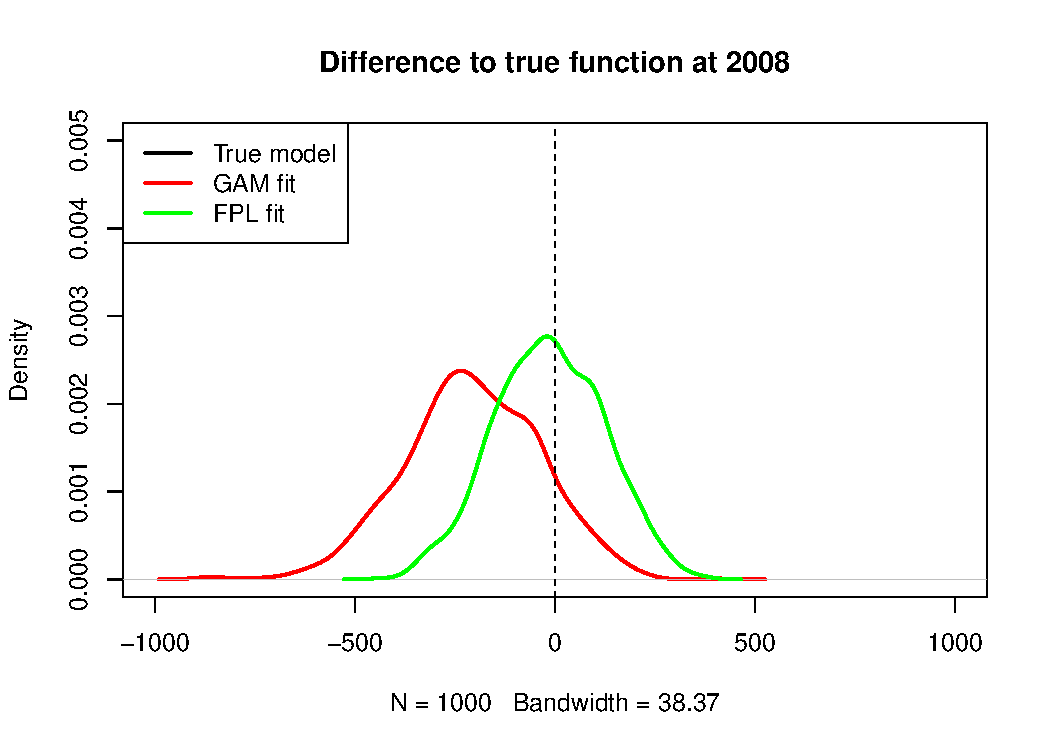
\includegraphics[width=1\linewidth]{figure/plot8-1} \hfill{}



\end{knitrout}
\caption{Distribution of the difference between the true model and the estimates of the GAM and FPL model at 2008.}
\label{fig:plot8}
\end{figure}


\begin{figure}
\begin{knitrout}
\definecolor{shadecolor}{rgb}{0.969, 0.969, 0.969}\color{fgcolor}\begin{kframe}
\begin{alltt}
\hlkwd{plot}\hlstd{(}\hlkwd{density}\hlstd{(out[,} \hlnum{2}\hlstd{]),} \hlkwc{main} \hlstd{=} \hlstr{"Difference to true function at 2017"}\hlstd{,}
    \hlkwc{xlim} \hlstd{=} \hlkwd{c}\hlstd{(}\hlopt{-}\hlnum{1000}\hlstd{,} \hlnum{1000}\hlstd{),} \hlkwc{ylim} \hlstd{=} \hlkwd{c}\hlstd{(}\hlnum{0}\hlstd{,} \hlnum{0.005}\hlstd{),}
    \hlkwc{col} \hlstd{=} \hlstr{"red"}\hlstd{,} \hlkwc{lwd} \hlstd{=} \hlnum{2}\hlstd{)}
\hlkwd{lines}\hlstd{(}\hlkwd{density}\hlstd{(out[,} \hlnum{4}\hlstd{]),} \hlkwc{col} \hlstd{=} \hlstr{"green"}\hlstd{,} \hlkwc{lwd} \hlstd{=} \hlnum{2}\hlstd{)}
\hlkwd{abline}\hlstd{(}\hlkwc{v} \hlstd{=} \hlnum{0}\hlstd{,} \hlkwc{lty} \hlstd{=} \hlnum{2}\hlstd{)}
\hlkwd{legend}\hlstd{(}\hlstr{"topleft"}\hlstd{,} \hlkwc{legend} \hlstd{=} \hlkwd{c}\hlstd{(}\hlstr{"True model"}\hlstd{,} \hlstr{"GAM fit"}\hlstd{,}
    \hlstr{"FPL fit"}\hlstd{),} \hlkwc{lwd} \hlstd{=} \hlnum{2}\hlstd{,} \hlkwc{col} \hlstd{=} \hlkwd{c}\hlstd{(}\hlstr{"black"}\hlstd{,} \hlstr{"red"}\hlstd{,}
    \hlstr{"green"}\hlstd{))}
\end{alltt}
\end{kframe}

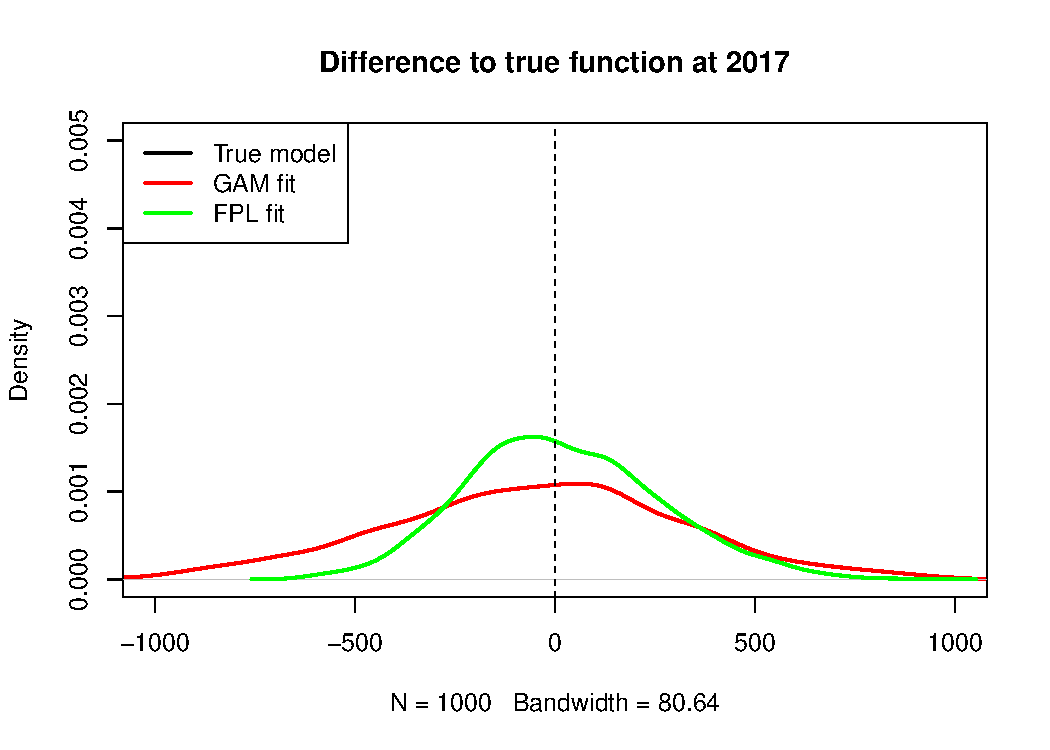
\includegraphics[width=1\linewidth]{figure/plot9-1} \hfill{}



\end{knitrout}
\caption{Distribution of the difference between the true model and the estimates of the GAM and FPL model at 2017.}
\label{fig:plot9}
\end{figure}


We see that GAM is negatively biased at 2008. The logistic model has no bias and lower variance at both time points. This is not very surprising because the true underlying model was also a logistic model.


\section{Conclusion}

We can conclude that GAM is a powerful tool to fit a curve to data which have some piecewise functional form. In our simulation, the logistic model was slightly better in fitting the true curve. However, the logistic model is much less flexible compared to GAM. Therefore, we recomend GAM as fast and easy to use model which can fit a wide variety of functions.


\bibliography{bib_packages}


\end{document}



